\documentclass{article}

  % packages
    % basic stuff for rendering math
    \usepackage[letterpaper, top=1in, bottom=1in, left=1in, right=1in]{geometry}
    \usepackage[utf8]{inputenc}
    \usepackage[english]{babel}
    \usepackage{amsmath} 
    \usepackage{amssymb}
    \usepackage{natbib}

    % extra math symbols and utilities
    \usepackage{mathtools}        % for extra stuff like \coloneqq
    \usepackage{mathrsfs}         % for extra stuff like \mathsrc{}
    \usepackage{centernot}        % for the centernot arrow 
    \usepackage{bm}               % for better boldsymbol/mathbf 
    \usepackage{bbm}              % for indicator functions
    \usepackage{enumitem}         % better control over enumerate, itemize
    \usepackage{hyperref}         % for hypertext linking
    \usepackage{xr-hyper}
    \usepackage{fancyvrb}         % for better verbatim environments
    \usepackage{newverbs}         % for texttt{}
    \usepackage{xcolor}           % for colored text 
    \usepackage{listings}         % to include code
    \usepackage{lstautogobble}    % helper package for code
    \usepackage{parcolumns}       % for side by side columns for two column code
    \usepackage{algorithm}
    \usepackage{algpseudocode}

    % page layout
    \usepackage{fancyhdr}         % for headers and footers 
    \usepackage{uniquecounter} 
    \usepackage{lastpage}         % to include last page number in footer 
    \usepackage{parskip}          % for no indentation and space between paragraphs    
    \usepackage[T1]{fontenc}      % to include \textbackslash
    \usepackage{footnote}
    \usepackage{etoolbox}

    % for custom environments
    \usepackage{tcolorbox}        % for better colored boxes in custom environments
    \tcbuselibrary{breakable}     % to allow tcolorboxes to break across pages

    % figures
    \usepackage{pgfplots}
    \pgfplotsset{compat=1.18}
    \usepackage{float}            % for [H] figure placement
    \usepackage{tikz}
    \usepackage{tikz-cd}
    \usepackage{circuitikz}
    \usetikzlibrary{positioning, shapes, arrows, fit, calc}
    \usepackage{graphicx}
    \usepackage{caption} 
    \usepackage{subcaption}
    \captionsetup{font=small}

    % for tabular stuff 
    \usepackage{dcolumn}

    \usepackage[nottoc]{tocbibind}
    \pdfsuppresswarningpagegroup=1
    \hfuzz=5.002pt                % ignore overfull hbox badness warnings below this limit

  % New and replaced operators
    \DeclareMathOperator{\Tr}{Tr}
    \DeclareMathOperator{\Sym}{Sym}
    \DeclareMathOperator{\Span}{span}
    \DeclareMathOperator{\elbo}{ELBO}
    \DeclareMathOperator{\std}{std}
    \DeclareMathOperator{\Cov}{Cov}
    \DeclareMathOperator{\Var}{Var}
    \DeclareMathOperator{\proj}{proj}
    \DeclareMathOperator{\Corr}{Corr}
    \DeclareMathOperator{\pos}{pos}
    \DeclareMathOperator*{\argmin}{\arg\!\min}
    \DeclareMathOperator*{\argmax}{\arg\!\max}
    \newcommand{\ket}[1]{\ensuremath{\left|#1\right\rangle}}
    \newcommand{\bra}[1]{\ensuremath{\left\langle#1\right|}}
    \newcommand{\braket}[2]{\langle #1 | #2 \rangle}
    \newcommand{\qed}{\hfill$\blacksquare$}     % I like QED squares to be black 

  % Custom Environments
    \newtcolorbox[auto counter, number within=section]{question}[1][]
    {
      colframe = orange!25,
      colback  = orange!10,
      coltitle = orange!20!black,  
      breakable, 
      title = \textbf{Question \thetcbcounter ~(#1)}
    }

    \newtcolorbox[auto counter, number within=section]{exercise}[1][]
    {
      colframe = teal!25,
      colback  = teal!10,
      coltitle = teal!20!black,  
      breakable, 
      title = \textbf{Exercise \thetcbcounter ~(#1)}
    }
    \newtcolorbox[auto counter, number within=section]{solution}[1][]
    {
      colframe = violet!25,
      colback  = violet!10,
      coltitle = violet!20!black,  
      breakable, 
      title = \textbf{Solution \thetcbcounter}
    }
    \newtcolorbox[auto counter, number within=section]{lemma}[1][]
    {
      colframe = red!25,
      colback  = red!10,
      coltitle = red!20!black,  
      breakable, 
      title = \textbf{Lemma \thetcbcounter ~(#1)}
    }
    \newtcolorbox[auto counter, number within=section]{theorem}[1][]
    {
      colframe = red!25,
      colback  = red!10,
      coltitle = red!20!black,  
      breakable, 
      title = \textbf{Theorem \thetcbcounter ~(#1)}
    } 
    \newtcolorbox[auto counter, number within=section]{proposition}[1][]
    {
      colframe = red!25,
      colback  = red!10,
      coltitle = red!20!black,  
      breakable, 
      title = \textbf{Proposition \thetcbcounter ~(#1)}
    } 
    \newtcolorbox[auto counter, number within=section]{corollary}[1][]
    {
      colframe = red!25,
      colback  = red!10,
      coltitle = red!20!black,  
      breakable, 
      title = \textbf{Corollary \thetcbcounter ~(#1)}
    } 
    \newtcolorbox[auto counter, number within=section]{proof}[1][]
    {
      colframe = orange!25,
      colback  = orange!10,
      coltitle = orange!20!black,  
      breakable, 
      title = \textbf{Proof. }
    } 
    \newtcolorbox[auto counter, number within=section]{definition}[1][]
    {
      colframe = yellow!25,
      colback  = yellow!10,
      coltitle = yellow!20!black,  
      breakable, 
      title = \textbf{Definition \thetcbcounter ~(#1)}
    } 
    \newtcolorbox[auto counter, number within=section]{example}[1][]
    {
      colframe = blue!25,
      colback  = blue!10,
      coltitle = blue!20!black,  
      breakable, 
      title = \textbf{Example \thetcbcounter ~(#1)}
    } 
    \newtcolorbox[auto counter, number within=section]{code}[1][]
    {
      colframe = green!25,
      colback  = green!10,
      coltitle = green!20!black,  
      breakable, 
      title = \textbf{Code \thetcbcounter ~(#1)}
    } 
    \newtcolorbox[auto counter, number within=section]{algo}[1][]
    {
      colframe = green!25,
      colback  = green!10,
      coltitle = green!20!black,  
      breakable, 
      title = \textbf{Algorithm \thetcbcounter ~(#1)}
    } 
    
    \definecolor{dkgreen}{rgb}{0,0.6,0}
    \definecolor{gray}{rgb}{0.5,0.5,0.5}
    \definecolor{mauve}{rgb}{0.58,0,0.82}
    \definecolor{darkblue}{rgb}{0,0,139}
    \definecolor{lightgray}{gray}{0.93}
    \renewcommand{\algorithmiccomment}[1]{\hfill$\triangleright$\textcolor{blue}{#1}}

    % default options for listings (for code)
    \lstset{
      autogobble,
      frame=ltbr,
      language=Python,                           % the language of the code
      aboveskip=3mm,
      belowskip=3mm,
      showstringspaces=false,
      columns=fullflexible,
      keepspaces=true,
      basicstyle={\small\ttfamily},
      numbers=left,
      firstnumber=1,                        % start line number at 1
      numberstyle=\tiny\color{gray},
      keywordstyle=\color{blue},
      commentstyle=\color{dkgreen},
      stringstyle=\color{mauve},
      backgroundcolor=\color{lightgray}, 
      breaklines=true,                      % break lines
      breakatwhitespace=true,
      tabsize=3, 
      xleftmargin=2em, 
      framexleftmargin=1.5em, 
      stepnumber=1
    }

  % Page style
    \pagestyle{fancy}
    \fancyhead[L]{Machine Learning}
    \fancyhead[C]{Muchang Bahng}
    \fancyhead[R]{Spring 2024} 
    \fancyfoot[C]{\thepage / \pageref{LastPage}}
    \renewcommand{\footrulewidth}{0.4pt}          % the footer line should be 0.4pt wide
    \renewcommand{\thispagestyle}[1]{}  % needed to include headers in title page

\begin{document}

\title{Factor and Component Models}
\author{Muchang Bahng}
\date{Spring 2025}

\maketitle
\tableofcontents
\pagebreak

\section{Principal Component Analysis} 
  
  PCA finds low dimensional approximations to the data by projecting the data onto linear subspaces. To begin with some motivation, let a linear map $A: \mathbb{R}^D \rightarrow \mathbb{R}^D$ be full rank, which maps some set of $n$ data points to the space of features. Then it is injective, and therefore for all data $x \in \mathbb{R}^D$ there exists a feature vector $z \in \mathbb{R}^D$ such that $z = Ax$. Generally, real-world data does not span the full space of $D$ dimensions.\footnote{The \textit{manifold hypothesis} that real-world data in high-dimensions actually lies on a lower-dimensional manifold. } In fact, if we further assume that the data lies in a linear subspace, we want to compress it into a lower-dimensional vector such that the covariates in this lower dimensional space are also orthogonal, i.e. uncorrelated. We tackle both problems in 2 steps. 
  \begin{enumerate}
    \item To compress this representation, we can take a data point $x \in \mathbb{R}^D$ and \textit{approximate} it as a point $\hat{x} \in L_k$ for some $k$-dimensional subspace $L_k \subset \mathbb{R}^d$ (say that this is done with some function $P: \mathbb{R}^D \rightarrow L_k \subset \mathbb{R}^D$). 
    \item After this projection, we then want to extract the $k$ features such that they are \textit{orthogonal} (i.e. no correlation). This is done with a simple change of basis, which we denote $T: L_k \rightarrow \mathbb{R}^k$, giving us $\hat{z} = T \hat{x} = T (P(x))$. We can invert this map $T^{-1} : \mathbb{R}^k \rightarrow L_k$ to go from the orthogonalized compressed version $\hat{z}$ to the approximate full version $\hat{x}$.
  \end{enumerate}
  We are done! But which subspace do we choose? Let's formalize what the optimal subspace should be. 

  \begin{definition}[Principal Subspace]
    Let $x \sim X \in \mathbb{R}^d$, with its normalized $\tilde{x} = x - \mathbb{E}[x]$, and $\mathcal{L}_k$ denote all $k$-dimensional linear subspaces of $\mathbb{R}^n$. The \textbf{$k$th principal subspace} is defined as 
    \begin{equation}
      \ell_k = \argmin_{\ell \in \mathcal{L}_k} \mathbb{E}_{\Tilde{x}} \big( \min_{y \in \ell} ||\Tilde{x} - y||^2 \big)
    \end{equation}

    To parse this, let's fix a subspace $\ell$. Then, the normalized data $\Tilde{x}$ is a random vector and the minimum distance of $\Tilde{x}$ onto the subspace $\ell$ is the inner min term. Taking the expectation of that gives us the expected distance of the data onto the subspace. The principal subspace is the subspace that minimizes this expected distance. The dimension reduced version of $x$ is then $P_k (x) = \mu + \mathrm{proj}_{\ell_k} x$. 

    \begin{figure}[H]
      \centering
      \begin{subfigure}[b]{0.4\textwidth}
      \centering
      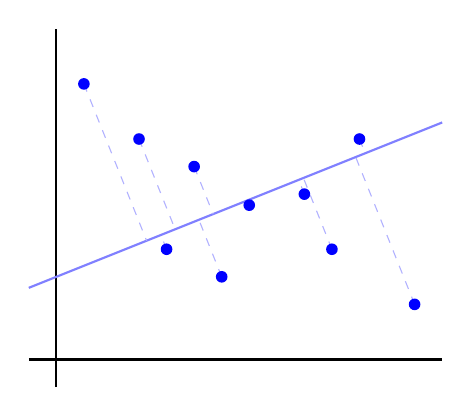
\begin{tikzpicture}[scale=0.7]
        % Draw axes
        \draw[black, line width=0.8pt] (-0.5,0) -- (7,0);
        \draw[black, line width=0.8pt] (0,-0.5) -- (0,6);
        
        % Define trend line coordinates (y = mx + b)
        \def\m{0.4}  % slope
        \def\b{1.5}  % y-intercept
        \draw[blue!50, line width=0.8pt] (-0.5,{-0.5*\m + \b}) -- (7,{7*\m + \b});
        
        % Calculate perpendicular direction vector (-m, 1) normalized
        \def\dx{-\m/sqrt(1+\m*\m)}
        \def\dy{1/sqrt(1+\m*\m)}
        
        % Points and their perpendicular projections
        % For point (x,y), intersection with line is:
        % x' = (x + m*y - m*b)/(1 + m^2)
        % y' = m*x' + b
        
        % Define and draw points with their projections
        \foreach \x/\y in {
          0.5/5,    % p1
          1.5/4,    % p2
          2/2,      % p3
          2.5/3.5,  % p4
          3/1.5,    % p5
          3.5/2.8,  % p6
          4.5/3,    % p7
          5/2,      % p8
          5.5/4,    % p9
          6.5/1     % p10
        } {
          % Calculate projection point
          \pgfmathsetmacro{\px}{(\x + \m*\y - \m*\b)/(1 + \m*\m)}
          \pgfmathsetmacro{\py}{\m*\px + \b}
          
          % Draw dashed line and point
          \draw[dashed, blue!30] (\x,\y) -- (\px,\py);
          \fill[blue] (\x,\y) circle (3pt);
        }
      \end{tikzpicture}
        \caption{PCA minimizes the orthogonal distance to the subspace. }
      \end{subfigure}
      \begin{subfigure}[b]{0.4\textwidth}
      \centering
      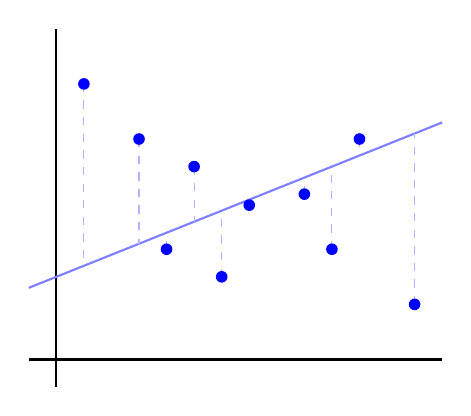
\begin{tikzpicture}[scale=0.7]
        % Draw axes
        \draw[black, line width=0.8pt] (-0.5,0) -- (7,0);
        \draw[black, line width=0.8pt] (0,-0.5) -- (0,6);
        
        % Define trend line function: y = 0.4x + 1.5
        \draw[blue!50, line width=0.8pt] (-0.5,1.3) -- (7,4.3);
        
        % Points with their actual trend line intersections
        \coordinate (p1) at (0.5,5);
        \path (0.5,1.7) coordinate (t1);  % trend point
        
        \coordinate (p2) at (1.5,4);
        \path (1.5,2.1) coordinate (t2);
        
        \coordinate (p3) at (2,2);
        \path (2,2.3) coordinate (t3);
        
        \coordinate (p4) at (2.5,3.5);
        \path (2.5,2.5) coordinate (t4);
        
        \coordinate (p5) at (3,1.5);
        \path (3,2.7) coordinate (t5);
        
        \coordinate (p6) at (3.5,2.8);
        \path (3.5,2.9) coordinate (t6);
        
        \coordinate (p7) at (4.5,3);
        \path (4.5,3.3) coordinate (t7);
        
        \coordinate (p8) at (5,2);
        \path (5,3.5) coordinate (t8);
        
        \coordinate (p9) at (5.5,4);
        \path (5.5,3.7) coordinate (t9);
        
        \coordinate (p10) at (6.5,1);
        \path (6.5,4.1) coordinate (t10);
        
        % Draw dashed lines from points to their trend line intersections
        \foreach \i in {1,...,10} {
          \draw[dashed, blue!30] (p\i) -- (t\i);
          \fill[blue] (p\i) circle (3pt);
        }
      \end{tikzpicture}
        \caption{Linear regression minimizes the residual distance to the subspace.} 
      \end{subfigure}
      \caption{Note that this is in fact different from linear regression as it minimizes the expected \textit{orthogonal distance} to the subspace, rather than the residual distance to the subspace as in linear regression.}
      \label{fig:pca_lin_reg}
    \end{figure}
  \end{definition}

  We can see that by definition the properties of the principal subspace allows us to construct the best approximation of the points in a lower-dimensional subspace. This seems like a hard optimization problem, but it turns out that the theorem gives a simple solution. Note that we need to do 3 things: 
  \begin{enumerate}
    \item Find such a subspace $\mathcal{L}_k \subset \mathbb{R}^D$. 
    \item Find the projection $P_k: \mathbb{R}^D \rightarrow \mathcal{L}_k \subset \mathbb{R}^D$. Note that by definition of the principal subspace $P_k$ should be an \textit{orthogonal} projection. 
    \item Find the bijection $T_k: \mathcal{L}_k \rightarrow \mathbb{R}^k$. 
  \end{enumerate}
  It turns out that we can solve all three problems with the singular value decomposition. 

  \begin{theorem}[Construction of the kth Principle Subspace] 
    Given covariates $x^{(1)}, \ldots, x^{(n)} \in \mathbb{R}^{d}$, let $X \in \mathbb{R}^{n \times d}$ be our random matrix representing our data, and its normalized form to $\Tilde{X} = X - \mu$. We take the SVD of it. 
    \begin{equation}
      \Tilde{X} = U \Sigma V^T
    \end{equation}
    where $U \in U(n) \subset \mathbb{R}^{n \times n}, V \in U(d) \subset \mathbb{R}^{d \times d}$ are orthogonal and $\Sigma \in \mathbb{R}^{n \times d}$ is diagonal that represents the singular values of $X$ in decreasing order\footnote{We can make it decreasing by permuting the rows/columns of the unitary matrices $U, V$.}. The columns of $V$ (rows of $V^T$) denoted $v_1, \ldots, v_d$ are called the \textbf{principal axes} and the columns of $U\Sigma$ are called the \textbf{principal components}. 
    \begin{enumerate}
      \item Then $\ell_k = \mathrm{span}\{v_1, \ldots, v_k\} \subset \mathbb{R}^d$, i.e. is the subspace spanned by the columns of $V$. By shifting it by $\mu$, $\mu + \ell_k$ is the best affine subspace approximation of the $x_i$'s. 

      \item The projection $P$ is defined 
      \begin{equation}
        \hat{x} = P_k (x) = \mu + \sum_{j=1}^k \langle x - \mu, v_j \rangle \, v_j = \sum_{j=1}^k \proj_{v_j} (x - \mu) = \mu + \proj_{\ell_k} (x - \mu)
      \end{equation}
      where we can rewrite it as the projection operator since the $v_j$'s are orthonormal. 

    \item The change of basis $T$ is defined with the mapping $\hat{x} \in \mathcal{L}_k \mapsto \sigma_j v_j \in \mathcal{L}_k$. Note that the $v_j$'s form an orthogonal basis of $\mathcal{L}_k$. 
    \end{enumerate} 
    Now let $V_k \in \mathbb{R}^{d \times k}$ represent the first $k$ columns of $V$ (aka first $k$ principal axes), $U_k \in \mathbb{R}^{n \times k}$ represent the first $k$ columns of $U$, and $\Sigma_k \in \mathbb{R}^{k \times k}$ represent the upper-left $k \times k$ matrix of $\Sigma$.\footnote{Note that $V^T$, which was originally surjective, is now just injective.} The product $U_k \Sigma_k$ represents the matrix containing the first $k$ principal components. The matrix $\Tilde{X}_k = U_k \Sigma_k V^T$, which is the low-rank approximation of $\Tilde{X}$, is called the \textbf{denoised matrix} of $\Tilde{X}$. 
  \end{theorem}
  \begin{proof}
    For notational convenience let $X = \Tilde{X}$. We see that 
    \begin{equation}
      X^T X =  V \Sigma^T \Sigma V^T
    \end{equation}
    Note that $X \neq V \Sigma^T$ in general. Now let $v_1, \ldots, v_d$ be the columns of $V$. Then 
    \begin{equation}
      X^T X [v_1, \ldots, v_d] = X^T X V = V \Sigma^T \Sigma = [\sigma_1^2 v_1, \ldots, \sigma_d^2 v_d]
    \end{equation}
    Therefore, we can see that the way $X^T X$ acts on $V$ That the $v_i$'s are the eigenvectors of $X^T X$, with $\sigma_i^2$ the associated eigenvalues. 
  \end{proof}

  Let's take a few moments to appreciate what $U$ and $V$ really represent. In some sense, $U_k \in \mathbb{R}^{n \times k}$ can be considered the dimension-reduced form of $\Tilde{X} \in \mathbb{R}^{n \times d}$. To see why consider the following. Let's label the \textit{rows} of $U_k$ as $u^{(1)}, \ldots, u^{(n)} \in \mathbb{R}^k$. By transposing the equation of the denoised matrix, we get $\Tilde{X}_k^T = V_k \Sigma_k U_k^T$, and so 
  \begin{equation}
    x^{(i)} - \mu = V_k \Sigma_k u^{(i)}
  \end{equation}
  for $i = 1, \ldots, n$. As an immediate consequence, since $T^{-1}$ maps $e_j$ to $\sigma_j v_j$, we can interpret $U_k \Sigma_k V_k^T$ with the decomposition 
  \begin{center}
    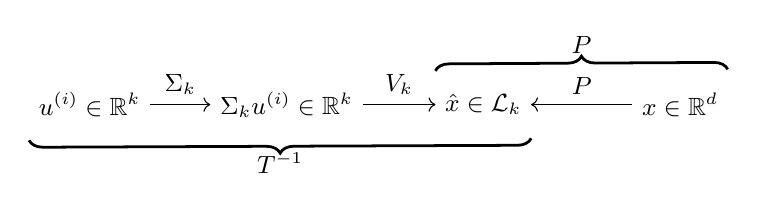
\begin{tikzpicture}[
      node distance=2.5cm,
      every node/.style={font=\small}
    ]
      % Nodes
      \node (vj) {$u^{(i)} \in \mathbb{R}^k$};
      \node[right of=vj] (sigmavj) {$\Sigma_k u^{(i)} \in \mathbb{R}^k$};
      \node[right of=sigmavj] (xhat) {$\hat{x} \in \mathcal{L}_k$};
      \node[right of=xhat] (x) {$x \in \mathbb{R}^d$};
      
      % Arrows
      \draw[->] (vj) -- node[above] {$\Sigma_k$} (sigmavj);
      \draw[->] (sigmavj) -- node[above] {$V_k$} (xhat);
      \draw[<-] (xhat) -- node[above] {$P$} (x);
      
      % Braces with increased thickness
      \draw[line width=1pt] [decoration={brace,mirror,raise=5pt,amplitude=5pt},decorate] (vj.south west) -- 
            node[below=6pt] {$T^{-1}$} (xhat.south east);
      \draw[line width=1pt] [decoration={brace,raise=5pt,amplitude=5pt},decorate] (xhat.north west) -- 
            node[above=7pt] {$P$} (x.north east);
    \end{tikzpicture}
  \end{center}

  This is very revealing. To embed the low-rank $u^{(i)}$ representation, it must go through some scaling $\Sigma_k$ followed by the injective map $V_k$. Now let's interpret $V_k$ and consider its \textit{columns}, labeled $v_1, \ldots, v_k \in \mathbb{R}^d$. These represent the basis vectors that span the subspace $\mathcal{L}_k$, i.e. the upscaled features in the higher-dimensional space. Therefore, $V_k$ represents the injection $e_i \in \mathbb{R}^k \mapsto v_i \in \mathcal{L}_k \subset \mathbb{R}^d$. This means that if we would like to pick a point with some combination of these features, we are really picking a point 
  \begin{equation}
    z = \sum_i z_i v_i \in \mathcal{L}_k
  \end{equation}

  \begin{algo}[Fitting] 
    Given a dataset $X \in \mathbb{R}^{n \times d}$, let us denote the rows as $x_i$, and say that we are looking for a subspace of dimension $k$. 
    \begin{enumerate}
      \item Compute the mean 
      \begin{equation}
        \mu = \frac{1}{n} \sum_{i=1}^n x_i  \in \mathbb{R}^d
      \end{equation} 

      \item Standardize the data $\Tilde{X} = X - \mu$, i.e. $\Tilde{x}_i = x_i - \mu$.  

      \item Compute the SVD $\Tilde{X} = U \Sigma V^T$.

      \item Compute the submatrices $V_k \in \mathbb{R}^{k \times k}$ and $\Sigma_k \in \mathbb{R}^{D \times k}$. 

      \item Define the projection operator $P_k (x) = \mu + \sum_{j=1}^k \langle x - \mu, v_j \rangle \, v_j$, the change of basis operator $T$, and the embedding operator $T^{-1} (z) = \mu + V_k \Sigma_k z$. 
    \end{enumerate} 
    A demonstration is done \href{code/pca.html}{here}.
  \end{algo}

  \begin{example}[Eigenfaces]
    In 1991, Turk and Pentland presented an eigenface method of face recognition by taking the low-rank approximation of a dataset of face images. 

    \begin{figure}[H]
      \centering 
      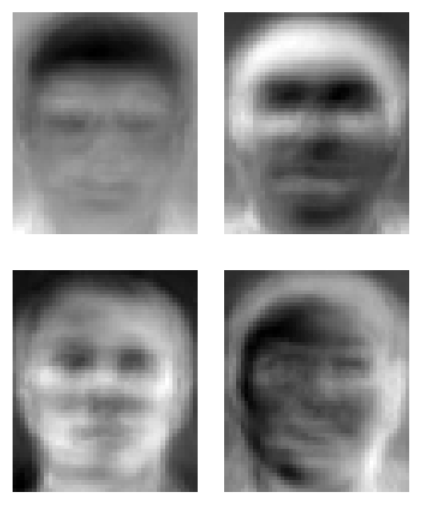
\includegraphics[scale=0.3]{img/eigenfaces.png}
      \caption{Some eigenfaces from AT\&T Labs. } 
      \label{fig:eigenfaces}
    \end{figure}
  \end{example}

  Now a question arises: how do we know that this sample decomposition is a good approximation to the true decomposition? It comes from the fact that the sample covariance $\hat{\Sigma}$ is a good approximation of the true covariance $\Sigma$, which we will later prove using concentration of measure. 

  \begin{theorem}[Risk]
    The risk satisfies 
    \begin{equation}
      R(k) = \mathbb{E}[|| x - P_k (x) ||^2 ] = \sum_{j=k+1}^D \lambda_j 
    \end{equation}
  \end{theorem}

  It is essential that you plot the spectrum in decreasing order. This allows you to analyze how well PCA is working. People often use the ``elbow'' technique to determine where to choose $K$, and we value 
  \begin{equation}
    \frac{\sum_{j=1}^k \lambda_j}{\sum_{j=1}^d \lambda_j} 
  \end{equation}
  accounts for the \textbf{variance explained}, which should be high with $K$ low. If you have to go out to dimension $K=50$ to explain $90\%$ of the variance, then PCA is not working. It may not work because of many reasons, such as there being nonlinear structure within the data. 

  It turns out that the elements of $\hat{\Sigma}$ are close entry-wise to those of $\Sigma$. But if this is true, then does it mean that the eigenvalues of the sample covariance matrix are close to the true eigenvalues of the covariance matrix? It turns out that the answer is no, and we need a proper metric to satisfy this assumption. The metric, as we can guess from linear algebra, is the operator norm, and we will show some results from matrix perturbation theory. 

  \begin{lemma}[]
    It turns out that 
    \begin{equation}
      ||\hat{\Sigma} - \Sigma|| = O_p \bigg( \frac{1}{\sqrt{n}} \bigg)
    \end{equation}
    where $|| \cdot ||$ is the operator norm. 
  \end{lemma}

  \begin{theorem}[Weyl's Theorem]
    If $\hat{\Sigma}$ and $\Sigma$ are close in the operator norm, then their eigenvalues are close. 
    \begin{equation}
      ||\hat{\Sigma} - \Sigma|| = O_p \bigg( \frac{1}{\sqrt{n}} \bigg) \implies |\hat{\lambda}_j - \lambda_j| = O_p \bigg( \frac{1}{\sqrt{n}} \bigg) 
    \end{equation}
  \end{theorem}

  This only talks about their eigenvalues, but this does not necessarily imply that the eigenvalues are close. We need an extra condition. 

  \begin{theorem}[David-Kahan Theorem]
    If $\hat{\Sigma}$ and $\Sigma$ are close in the operator norm, and if the eigenvectors of $\Sigma$ are well-conditioned, then the eigenvectors of $\hat{\Sigma}$ are close to the eigenvectors of $\Sigma$. More specifically, 
    \begin{equation}
      ||\hat{v}_j - v_j|| \leq \frac{2^{3/2} ||\hat{\Sigma} - \Sigma||}{\lambda_j - \lambda_{j+1}}
    \end{equation}
  \end{theorem}

\subsection{Kernel PCA}

  \begin{definition}[Kernel PCA]
    Let $N_i$ be the neighborhood around $X_i$. Then, we want to find a mapping $W: \mathbb{R}^n \rightarrow \mathbb{R}^k$ that minimizes 
    \begin{equation}
      \min_{W} \sum_{i=1}^n \bigg| \bigg| X_i - \sum_{j \in N_i} W_{ij} X_j \bigg| \bigg|^2 \text{ where } \sum_{j} W_{ij} = 1
    \end{equation}
    We can constrain the weights in $W$ so that anything that is not in the neighborhoods are $0$. 
  \end{definition}

\section{Linear Latent Variable Models}

  Note that in PCA, we have taken some data $x$ in high-dimension $D$ and reduced it to a lower-dimensional orthogonal representation in $\mathbb{R}^k$. In other words, the corresponding $z$ represents $x$ in another space, which we call a \textbf{latent space}. A model that represents data from the original space $\mathcal{X}$ to a latent space $\mathcal{Z}$ is called a \textit{latent variable model}. We will extend on this. 

  Say that we have some covariates $x^{(i)} \sim X$ and we want to find its true distribution $p^\ast$. In density estimation so far, what we have done is define a family of distributions $\{p_\theta\}$ and optimize the loss by maximizing the MLE or something else. 
  \begin{equation}
    \min_\theta L(p_\theta, p^\ast) = \max_\theta \prod_{i} p_\theta(x^{(i)})
  \end{equation}
  In order to do this we work with explicitly parameterized distribution families (e.g. Gaussian, Gamma, multinomial, etc.), but this is too simple to model complex things in real like (e.g. the distribution of faces). Therefore, we consider \textit{implicitly parameterized} probability distributions by ``adding'' a latent distribution $Z$, creating the joint distribution $(X, Z)$. This may look more complicated, but it captures a much richer family of distributions. 

  \begin{definition}[Generative Latent Variable Model]
    A \textbf{latent variable model} is a model of a distribution $p^\ast (x)$ over a space $\mathcal{X}$ using implicitly parameterized probability distributions $p_\theta$ constructed as such: 
    \begin{enumerate}
      \item We define a simple random variable $Z$ over $\mathcal{Z}$ with its distribution $p(z)$, called the \textbf{prior}.\footnote{Almost always a uniform or normal distribution suffices. If not, we can constrain it to be factorable (i.e. is the product of its marginal distributions: $p(z) = \prod_i p(z_i)$) so that it is easy to sample from. Occasionally, the stronger assumption of the $z_i$'s being iid is made. } 
      \item We define a family of functions $\{f_\theta\}$ defined over $z$ and parameterized by $\theta$. 
      \item We define a way to convert any $f_\theta(z)$ into a distribution $p(x \mid z)$, called the \textbf{likelihood} or \textbf{generative component}. There are generally two ways to do this: 
      \begin{enumerate}
        \item Let the random variable $X \mid Z = z$ be an explicitly parameterized distribution, and have $f_\theta (z)$ be the parameters of $X \mid Z = z$. Therefore, we take the output of $f_\theta (z)$ and plug in these values as the parameters of $X \mid Z = z$.\footnote{For example, let $f_\theta (z) = (f_1 (z), f_2(z))$. Then we define the corresponding distribution $X \mid Z = z \sim \mathcal{N}(f_1 (z), e^{f_2 (z)} )$.}
        \item Have $f_\theta$ be a transformation of random variables, i.e. $X = f(Z)$. This may result in a conditional pdf that is not explicitly parameterizable.
      \end{enumerate}
    \end{enumerate}
    This defines the family of joint distributions $p_\theta$ over $(\mathcal{Z}, \mathcal{X})$. It is easy to sample $(x, z) \sim p_\theta$: sample $z \sim p$, then compute $f_\theta (z)$, use this to define $p_\theta (x \mid z)$, and finally sample from the likelihood. Therefore, the joint is also of a simple nature. 

    While we assume simple, explicitly parameterized forms for the prior and the likelihood, we do not assume anything about 
    \begin{enumerate}
      \item the \textbf{marginal} $p_\theta (x)$. Usually this is an extremely complicated distribution, which is equivalent to 
      \begin{equation} 
        p_X (x) = \int_{z \in \mathbb{R}^k} p (x \mid z) \, p_Z (z) \,dz = \mathbb{E}_Z [p(X \mid Z)] 
      \end{equation} 
      from marginalizing but is computationally impossible to integrate. 

      \item the \textbf{posterior} $p_\theta (z \mid x)$ that describes the hidden features given some data point. This is also known as the \textbf{inference component}. By Bayes rule, we have 
      \begin{equation}
        p_\theta (z \mid x) = \frac{p_\theta (x \mid z) \, p(z)}{p_\theta (z \mid x)} \iff p_\theta (z \mid x) \propto p_\theta (x \mid z) \, p(z)
      \end{equation}
      which we might be able to sample from using MCMC. 
    \end{enumerate}
  \end{definition} 

  Like we do with everything else in math, we take a look at the simplest example: when the class $\{f_\theta\}$ are linear functions that represent \textit{transformations}\footnote{Not have its output parameterize $X \mid Z = z$.} $X = f(Z)$ of the random variable $Z$. This is known as \textbf{linear latent variable modeling}. 
  \begin{equation}
    X = \mu + W Z + \epsilon
  \end{equation}
  where the noise $\epsilon$ is typically Gaussian and diagonal (but not necessarily the same component-wise variances). Finally, we can use techniques like MLE to estimate $W, \mu$, and the parameters of $\epsilon$. The entire reason we want to do this is that we are hoping that we can construct a complex distribution $X$ from a simple distribution $Z$ with $d >> k$, connected by some well-studied function $X = f(Z)$. In the linear case, $W \in \mathbb{R}^{d \times k}$, and the latent variables $z$ give a more compact, parsimonious  explanation of dependencies between the components of the observations $x$. 

  \begin{definition}[Factor Analysis] 
    \textbf{Factor analysis} is a specific case of a linear latent variable model where 
    \begin{equation}
      X = \mu + WZ + \epsilon, \text{ where } z \in \mathcal{N}(0, I), \epsilon \sim \mathcal{N} \big(0, \mathrm{diag}(\sigma_1^2, \ldots, \sigma_k^2) \big)
    \end{equation}
    It should be clear to us that $X$ should be Gaussian\footnote{Since linear transformations of Gaussians are Gaussian} and that $\mathbb{E}[X] = \mu$, with 
    \begin{align} 
        \mathrm{Var}[X] & = \mathbb{E}[ (X - \mu)(X - \mu)^T ] \\
                        & = \mathbb{E}[ (W Z + \epsilon) (Z^T W^T + \epsilon^T)] \\
                        & = \mathbb{E}[W z z^T W^T] + \mathbb{E}[ \epsilon \epsilon^T] \\
                        & = W \mathbb{E}[ z z^T] W^T + \mathbb{E}[ \epsilon \epsilon^T] \\
                        & = W W^T + \mathrm{diag}(\sigma_1^2, \ldots, \sigma_d^2) 
    \end{align} 
    The $W, \mu$, and $\sigma_i$'s can be estimated using MLE methods. 
  \end{definition} 

\subsection{Probabilistic PCA}

  We want to take PCA and extend it to be a \textit{generative model}, which allows you to sample data. In regular PCA, we saw that for some $z \in \mathbb{R}^k$ in the latent space, $\hat{x} = \mu + V_k \Sigma_k z$. Therefore, if we just change $z$ from a point to a probability distribution (e.g. Gaussian), we can take a random variable $z \sim \mathcal{N}(0, I)$ from $\mathbb{R}^k$, and then transform it to get a random variable $x = \mu + U_k \Sigma_k z$, which will give a density. 
  \begin{equation}
    x \sim \mathcal{N} \big( \mu, (V_k \Sigma_k)(V_k \Sigma_k)^T \big) = \mathcal{N} \big( \mu, V_k \Sigma_k U_k^T U_k \Sigma_k V_k^T \big) = \mathcal{N} \big( \mu, X_k^T X_k)
  \end{equation} 
  Note that in here, $x$ is a random variable that we are trying to fit to the data $X_k$. However, $X_k \in \mathbb{R}^{n \times d}$ with $d << n$, and so $X_k^T X_k \in \mathbb{R}^{d \times d}$ is not full rank, and so the distribution is restricted to strictly the $k$-dimensional subspace $L_k \subset \mathbb{R}^D$. We want to add a bit of noise beyond the subspace, so we add an extra small Gaussian $\epsilon$ around it. In general factor analysis above, we set $\epsilon$ to have an arbitrary diagonal Gaussian, but for PPCA we just use an isotropic one $\epsilon \sim \mathcal{N}(0, \sigma^2 I)$, giving us  
  \begin{equation}
    x = \mu + U_k \Sigma_k z + \epsilon \implies X \sim \mathcal{N}(\mu, X_k^T X_k + \sigma^2 I)
  \end{equation} 
  Now rather than treating $X_k^T$ as a data matrix that we use to calculate the principal subspace, we treat it as a parameter matrix $W \in \mathbb{R}^{d \times n}$ that we want to fit \cite{ppca}. Note that PPCA is really a specific instance of factor analysis, and we assume that the latent variable $z$ follows a standard Gaussian $\mathcal{N}(0, 1)$. 

  \begin{definition}[Probabilistic PCA] 
    The \textbf{probabilistic PCA} model is a latent factor model with $Z \sim \mathcal{N}(0, I)$ and 
    \begin{equation}
      X = f_\theta (Z) = \mu + (WW^T + \sigma^2 I )^{1/2} Z
    \end{equation}
    and $\theta = \{\mu, W, \sigma\}$, which gives
    \begin{equation}
      X \sim \mathcal{N}(\mu, W W^T + \sigma^2 I) 
    \end{equation} 
  \end{definition} 

  Optimizing this model is actually quite easy. 

  \begin{theorem}[MLE of PPCA Model]
    Given $x^{(i)} \sim X$ iid, the MLEs for $W, \mu, \sigma$ are 
    \begin{align}
      \mu_{MLE} & = \frac{1}{N} \sum_{i=1}^N x^{(i)} \implies \hat{\mu}_{MLE} = \frac{1}{N} \sum_{i=1}^N x^{(i)} \\ 
      \hat{\sigma}^2_{MLE} & = \frac{1}{d-k} \sum_{j=k+1}^d \lambda_j \\
      W_{MLE} & = U_q (\Lambda_d - \hat{\sigma}_{MLE}^2 I_d )^{1/2} R
    \end{align}
  \end{theorem}
  \begin{proof}
    Given $x^{(i)} \sim X$ iid, the MLEs for $W, \mu, \sigma$ have a closed form, and model parameter estimation can be performed iteratively and efficiently. We have 
    \begin{equation}
      \mu_{MLE} = \frac{1}{N} \sum_{i=1}^N x^{(i)} \implies \hat{\mu}_{MLE} = \frac{1}{N} \sum_{i=1}^N x^{(i)}
    \end{equation}
    and setting the biased MLE estimator of the variance, 
    \begin{equation}
      \widehat{\mathrm{Var}}_{MLE}(\mu_{MLE}) = S = \frac{1}{N} \sum_{i=1}^N (x^{(i)} - \mu_{MLE}) (x^{(i)} - \mu_{MLE})^T
    \end{equation}
    we can derive the MLE of $W$.\footnote{Note that $W_{MLE}$ is not unique. Say that $W^\ast$ is an MLE, then, for any unitary $U \in \mathbb{R}^{k \times k}$, we have $W^\ast W^{\ast T} = (W^\ast U) (W^\ast U)^T$.} We can find the MLE estimate of $\sigma$ first by taking a look at $C = \mathrm{Var}[X] = W W^T + \sigma^2 I$. It is the sum of positive semidefinite patrices that are also symmetric, so by the spectral theorem it is diagonalizable and has full rank $d$. But $W W^T$ is rank $k$, so $d - k$ of the eigenvalues of $W W^T$ is $0$, indicating that the same $d-k$ smallest eigenvalues of $C$ is $\sigma^2$. Therefore, we can take the smallest $d-k$ eigenvalues of our MLE estimator of $C$, which is $S$, and average them to get our MLE for $\sigma$. 
    \begin{equation}
      \hat{\sigma}^2_{MLE} = \frac{1}{d-k} \sum_{j=k+1}^d \lambda_j
    \end{equation}
    We can approximate $W W^T = C - \sigma^2 I \approx S - \hat{\sigma}^2_{MLE} I$, and by further taking the eigendecomposition $C = U \Sigma U^T \implies W W^T = U (\Sigma - \sigma^2 I) U^T$ and cutting off the last $d-k$ smallest eigenvalues and their corresponding eigenvectors, we can get 
    \begin{equation}
      W_{MLE} = U_q (\Lambda_d - \hat{\sigma}_{MLE}^2 I_d )^{1/2} R
    \end{equation}
    where the $R$ just accounts for any unitary matrix. 
  \end{proof}

  Now as $\sigma \rightarrow 0$, the density model defined by PPCA becomes very sharp around these $d$ dimensions spanned by the columns of $W$. At $0$, our MLE of $W$ is simplified and we have 
  \begin{equation}
    X = W_{MLE} z + \mu_{MLE} + \epsilon = U_q \Lambda_q^{1/2} z + \mu_{MLE}
  \end{equation}
  which essentially reduces to regular PCA. That is, the conditional expected value of $z$ given $X$ becomes an orthogonal projection of $X - \mu$ onto the subspace spanned by the columns of $W$. Intuitively, we can see that we are estimating the Gaussian, which corresponds to the mean squared distance from each $x^{(i)}$ to $\ell_k$. 

\subsection{Linear Independent Component Analysis} 

  ICA is a method to separate a multivariate signal into additive, statistically independent components. It does come with a lot of assumptions, and is a specific instance of a linear factor model where $\mu = 0$ and $\epsilon = 0$. 

  \begin{definition}[Linear ICA]
    In \textbf{linear ICA}, we have the simple model. 
    \begin{equation}
      x = W z
    \end{equation}
    In here, $X \in \mathbb{R}^d$ is a mixture vector and $W \in \mathbb{R}^{d \times k}$ is a \textbf{mixing matrix}. Both $W$ and $z$ are unknown, and we need to recover them given $x$. We have 2 strong assumptions. 
    \begin{enumerate} 
      \item Each component of $z$ is independent (not just uncorrelated). This is an easy enough assumption to intuit.  
      \item Independent components of $z$ must \textit{not} be Gaussian.\footnote{This is needed for us to be able to ``unmix'' the signals. To see why, just suppose $z$ was Gaussian, and so the vector $Rz$ is also Gaussian for any invertible $R$. Therefore, we could find an infinite number of solutions of form $x = W R^{-1} R z$ and have no way to separate them.}
    \end{enumerate}
  \end{definition}

  \begin{algo}[Fitting]
    Now let's see how linear ICA actually estimates $W$ and $z$. Once $W$ is estimated, the latent components of a given test mixture vector, $x^\ast$ is computed by $z^\ast = W^{-1} x^\ast$. So now all there's left to do is to estimate $W$, which we want to estimate so that $W^{-1} x$ is far from Gaussian. The reason for this is that given a bunch of independent non-Gaussian $h_i$'s, if we mix them with a matrix that is not $\pm I$ , then by CLT, a linear combination of random variables will tend to be Gaussian, and so for an arbitrary $W$ we would expect $x$ to be Gaussian. Therefore, what we want to do is guess some matrix $A$, and compute 
    \begin{equation}
      A x = A W h
    \end{equation}
    and if we get things right, $A \approx W^{-1}$, and the result of $A x$ would look pretty non-Gaussian. If it it not the case, then $A W$ will still be some mixing matrix, and so $A x$ would look Gaussian. So now the question reduces to how do we choose this $A$? There are multiple ways to measure non-Gaussianity: 
    \begin{enumerate} 
      \item The absolute or squared kurtosis, which is $0$ for Gaussians. This is a differentiable function w.r.t. $W$, so we can try maximizing it. This is done for the sample kurtosis, of course.  
      \item Another measure is by maximizing the neg-entropy. 
    \end{enumerate}
  \end{algo}

  There are further ambiguities with ICA regarding uniqueness of a best representation. For one, we can only estimate the latent components up to a scaling factor since we will still get
  \begin{equation}
    x = (\alpha W) (\frac{1}{\alpha} z) \text{ for some } \alpha > 0
  \end{equation}
  We can fix this by forcing $\mathbb{E}[z_i^2] = 1$. However, there is still an ambiguity for the sign of hidden components, but this is insignificant in most applications. Second, we can estimating the components up to permutation. We have 
  \begin{equation}
    x = W P^{-1} P z
  \end{equation}
  for some permutation matrix $P$. 

  \begin{figure}[H]
    \centering 
    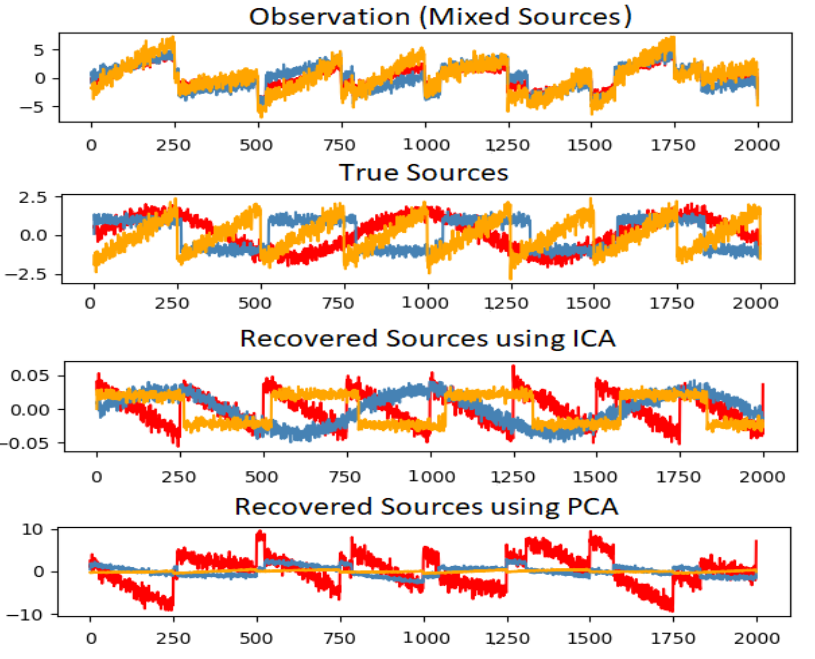
\includegraphics[scale=0.4]{img/ICA_example.png}
    \caption{We can perform this on three mixed signals with additive noise, and ICA does very well, though again some recovered signals are scaled or permuted weirdly. }
    \label{fig:}
  \end{figure}

\subsection{Slow Feature Analysis}

  Slow feature analysis also another special case of a linear factor model that uses information from time signals to learn invariant features. It is motivated by a general principle called the \textbf{slowness principle}. The idea is that the important characteristics of scenes change very slowly compared to the individual measurements that make up a description of a scene. For example, in computer vision, individual pixels can change very rapidly. If a zebra moves from left to right across the image, an individual pixel wil rapidly change from black to white. By comparison, the feature indicating whether a zebra is in the image will not change at all, and the feature describing the zebra's position will change slowly. Therefore, we want to regularize our model to learn features that change slowly over time.  

  We can apply the slowness principle to any differentiable model trained with gradient descent. That is, we can add the following term to the loss function: 
  \begin{equation}
    \lambda \sum_i d\big( f(x^{(t+1)}), f(x^{(t)}) \big)
  \end{equation}
  where $\lambda$ is a hyperparameter determining the strength of the slowness regularization term, $t$ is the time index, $f$ is the feature extractor to be regularized, and $d$ is the distance between $f(x^{(t)})$ and $f(x^{(t+1)})$. A common choice for $d$ is the mean squared difference. 

  Essentially, given a set of time-varying input signals $x^{(t)}$, SFA learns a nonlinear function $f$ that transforms $x$ into slowly-varying output signals $y$. Obviously, we can't just take some trivial function like $f = 0$, so we have the following constraints 
  \begin{align}
    \mathbb{E}_t [ f(x^{(t)})_i]  & = 0 \\ 
    \mathbb{E}_t [ f(x^{(t)})_i^2] & = 1 
  \end{align}
  \begin{center} 
    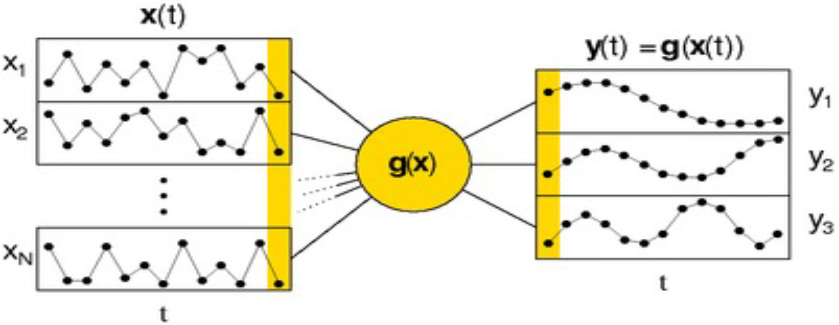
\includegraphics[scale=0.4]{img/slow_feature.png}
  \end{center}
  We can restrict the nonlinear $f$ to some subspace of functions, and this becomes a standard optimization problem where we solve 
  \begin{equation}
    \min_\theta \mathbb{E}_t \big[ \big( f(x^{(t+1)})_i - f(x^{(t)})_i \big)^2 \big]
  \end{equation}

\subsection{Latent Dirichlet Allocation} 

\subsection{Sparse Dictionary Learning} 

  Latent variables can help us represent data in lower dimensions, but another advantage is that we can get \textit{sparse} representations as well. What we want to do in sparse coding is that for each input $x^{(i)}$, we want to find a latent representation $z^{(i)}$ such that it is sparse (i.e. has many $0$s) and also we can reconstruct the original input $x^{(i)}$ well. We have basically two things to optimize: the latent representations $z$ and the decoding mechanism, which we can do with a \textit{dictionary matrix} $D$. Note that we are optimizing for \textit{both} the latent encodings and the decoding mechanism, and so this isn't a generative model. 

  \begin{definition}[Sparse Dictionary Encoding Model]
    The \textbf{sparse dictionary encoding model} is a representation model defined 
    \begin{equation}
      X = g_{D}(Z) = D Z
    \end{equation}
    where $D \in \mathbb{R}^{d \times k}$ is a \textbf{dictionary matrix} that decodes the latent $Z \in \mathbb{R}^k$ to $X \in \mathbb{R}^d$. Note that both the $z^{(i)}$'s and $D$ are optimized, so we want to perform the \textit{joint} optimization\footnote{To break this term down, let's just assume that we have a fixed dictionary $D$. Then, we just need to minimize with respect to each $h^{(t)}$. Now we can add the dictionary parameter back again. }

    \begin{equation}
      \min_{D} \frac{1}{N} \sum_{i=1}^N \min_{z^{(i)}} \underbrace{\frac{1}{2} ||x^{(i)} - D z^{(i)}||_2^2}_{\text{reconstruction error}} + \underbrace{\lambda ||z^{(i)}||_1}_{\text{sparsity penalty}}
    \end{equation}
  \end{definition}

  Note that the reconstruction, or decoding, of $x = Dz$ is linear and explicit, but if we want to encode $x \mapsto z$, we need to substitute the $x$ into the term above and minimize it w.r.t. $D$ and $z$ to solve it. Therefore, this encoder is an implicit and \textit{nonlinear} function of $x$. 

  \begin{figure}[H]
    \centering 
    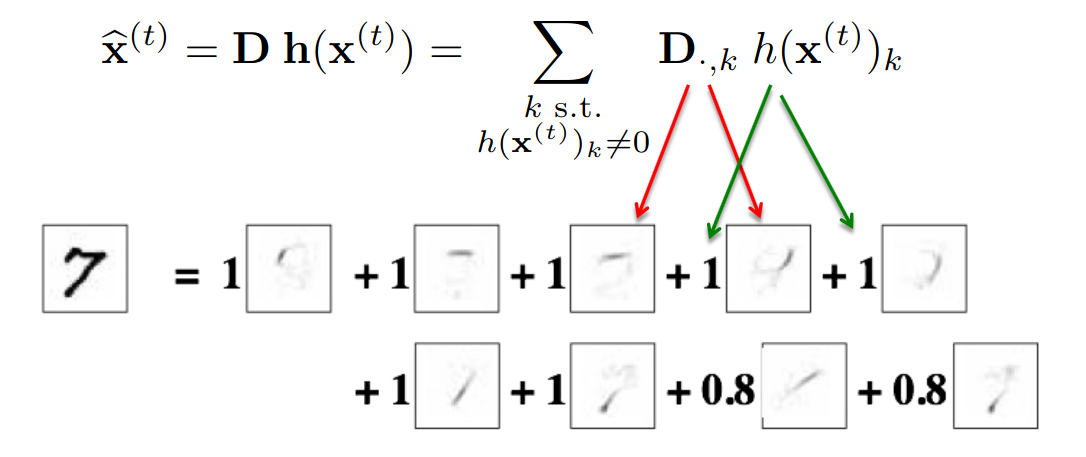
\includegraphics[scale=0.4]{img/sparse_coding.png}
    \caption{We can reconstruct an image of a seven as a linear combination of a set of images. Note that each of the images of strokes are columns of $W$ and the coefficients make up the sparse vector $h$. } 
    \label{fig:sparse_coding}
  \end{figure}

  Let's think about how we can optimize the objective function w.r.t. $h$, keeping $D$ constant. We can do stochastic gradient descent, which gives us the steps
  \begin{equation}
    \nabla_{h^{(t)}} \mathcal{L}(x^{(t)}) = D^T (D h^{(t)} - x^{(t)}) + \lambda \, \mathrm{sign}(h^{(t)})
  \end{equation}
  but this wouldn't achieve sparsity since it overshoots the $0$ all the time. Therefore, we can clip it, or we can use proximal gradient descent/ISTA to take a step, and shrink the parameters according to the L1 norm. 
  \begin{align} 
    h^{(t)} & = h^{(t)} - \alpha D^T (D h^{(t)} - x^{(t)}) \\
    h^{(t)} & = \mathrm{shrink}(h^{(t)}, \alpha \lambda)
  \end{align}
  where $\mathrm{shrink}(a, b) = [\ldots, \mathrm{sign}(a_i)\, \max(|a_i| - b_i, 0), \ldots]$. This is guaranteed to converge if $1/\alpha$ is bigger than the largest eigenvalue of $D^T D$.  


\bibliography{./bibfile}
\bibliographystyle{alpha}

\end{document}
